% Explain the implementaiton of the debug adapeter

% Overview description of the debug adapter and the flow of communication from the user to the debugger.
The debug adapter is implemented as a \gls{tcp} server in the main thread.
When a new \gls{tcp} connection is made the debug thread is started.
After it has started the main thread starts listening for \gls{dap} messages on the \gls{tcp} connection.


The first \gls{dap} messages are for communicating the \gls{dap} functionalities that the client and the debugger has.
These first \gls{dap} messages also contain some configuration for debugger module in the debug thread, those configuration are forwarded to the debug thread.
After that the debug adapter will continuously pull for messages from the \gls{tcp} client and the debug thread, until a message is received.


When the debug adapter receives a \gls{dap} message from the client it is translated into one or more commands.
Those commands are then sent one by one to the debugger module in the debug thread.
The responses from those commands are then used to make a response to the clients \gls{dap} message.
If the debug adapter gets a event from the debug thread it will translate it into a \gls{dap} message and send it to the client.



%% Add a flow cart of the communication? % TODO
%\begin{figure}[h]
%	\centering
%	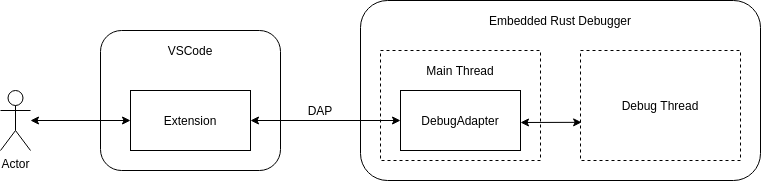
\includegraphics[width=0.9\textwidth]{user_dap_debug.png}
%	\caption{A diagram showing the comunication between the user/actor, \emph{VSCode} and the debugger \emph{Embedded Rust Debugger}.}
%	\label{fig:userDAP}
%\end{figure}


